\documentclass[final]{article}

\usepackage[utf8]{inputenc}
\usepackage[T1]{fontenc}
\usepackage[a1paper,landscape,margin=18mm]{geometry}
\usepackage{graphicx}
\usepackage{booktabs}
\usepackage{array}
\usepackage{multicol}
\usepackage{ragged2e}
\usepackage{enumitem}
\usepackage{xcolor}
\usepackage{tikz}
\usetikzlibrary{arrows.meta,positioning}
\usepackage[hidelinks]{hyperref}

\pagestyle{empty}
\setlength{\parindent}{0pt}
\setlength{\parskip}{6pt}
\renewcommand{\familydefault}{\sfdefault}

\definecolor{MycoGreen}{HTML}{1F7A5D}
\definecolor{MycoGreenDark}{HTML}{15533F}
\definecolor{MycoMint}{HTML}{E8F6F1}
\definecolor{MycoBlue}{HTML}{1F4E79}
\definecolor{MycoBlueLight}{HTML}{EAF2FB}
\definecolor{MycoGold}{HTML}{B07D12}
\definecolor{MycoGoldLight}{HTML}{FFF6E3}
\definecolor{MycoGray}{HTML}{4B5563}
\definecolor{MycoBorder}{HTML}{BFD7CF}

\newcommand{\postersection}[2]{%
  \vspace{1mm}%
  {\Large\bfseries\color{MycoGreenDark} #1}\par
  \vspace{2mm}%
  {\large #2}
}

\newcommand{\statcard}[3]{%
  \begin{minipage}[t]{0.235\textwidth}
    \fcolorbox{MycoBorder}{#2}{%
      \begin{minipage}[t][4.9cm][c]{0.965\linewidth}
        \centering
        {\fontsize{28}{32}\selectfont\bfseries #1}\par
        \vspace{1mm}
        {\large\bfseries\color{MycoGreenDark} #3}
      \end{minipage}%
    }
  \end{minipage}
}

\newcommand{\contentbox}[2]{%
  \fcolorbox{MycoBorder}{#1}{%
    \begin{minipage}[t]{0.96\linewidth}
      \vspace{4mm}
      \hspace{4mm}
      \begin{minipage}[t]{0.92\linewidth}
        #2
      \end{minipage}
      \vspace{4mm}
    \end{minipage}%
  }
}

\begin{document}

\begin{center}
  {\fontsize{44}{52}\selectfont\bfseries\color{MycoGreenDark}
  MycoFlow: Bio-Inspired Reflexive QoS for OpenWrt Routers}\par
  \vspace{4mm}
  {\Large A1 poster draft for project introduction and academic presentation}\par
  \vspace{3mm}
  {\large Bar\i{}s Can Atakl\i{} \quad $\cdot$ \quad MycoFlow Core Project \quad $\cdot$ \quad \href{https://github.com/bariscanatakli/mycoflow-core}{github.com/bariscanatakli/mycoflow-core}}\par
\end{center}

\vspace{4mm}

\begin{center}
  \statcard{154$\times$}{MycoGoldLight}{lower average in-tin delay for gaming traffic vs. bulk}
  \hfill
  \statcard{38\%}{MycoBlueLight}{gaming latency reduction under five mixed-persona clients}
  \hfill
  \statcard{66.97\%}{MycoMint}{CAKE tin accuracy on observed flows in vivo}
  \hfill
  \statcard{0}{MycoGoldLight}{flash writes during runtime}
\end{center}

\vspace{5mm}

\noindent
\begin{minipage}[t]{0.31\textwidth}
  \contentbox{MycoMint}{
    \postersection{The problem}{
      Consumer routers must serve gaming, VoIP, video calls, and bulk transfers at the same time.
      Static QoS settings cannot react to changing traffic patterns, and most traffic arrives unmarked,
      so CAKE often sees everything as best-effort.
    }

    \vspace{3mm}
    \postersection{What MycoFlow does}{
      \begin{itemize}[leftmargin=*,itemsep=2pt,topsep=0pt]
        \item Infers per-device persona and per-flow service class on-device.
        \item Marks flows with DSCP and steers them into CAKE diffserv tins.
        \item Adjusts bandwidth and policy using a 1 Hz Sense$\to$Infer$\to$Act$\to$Stabilize loop.
        \item Keeps all mutable state in RAM or tmpfs, not flash.
      \end{itemize}
    }

    \vspace{2mm}
    \postersection{Why it matters}{
      The system targets the exact constraints of embedded OpenWrt hardware: low CPU, low RAM, and no cloud offload.
      This makes application-aware QoS practical on consumer routers instead of only on enterprise gear.
    }
  }
\end{minipage}
\hfill
\begin{minipage}[t]{0.35\textwidth}
  \contentbox{MycoBlueLight}{
    \postersection{How it works}{
      \centering
      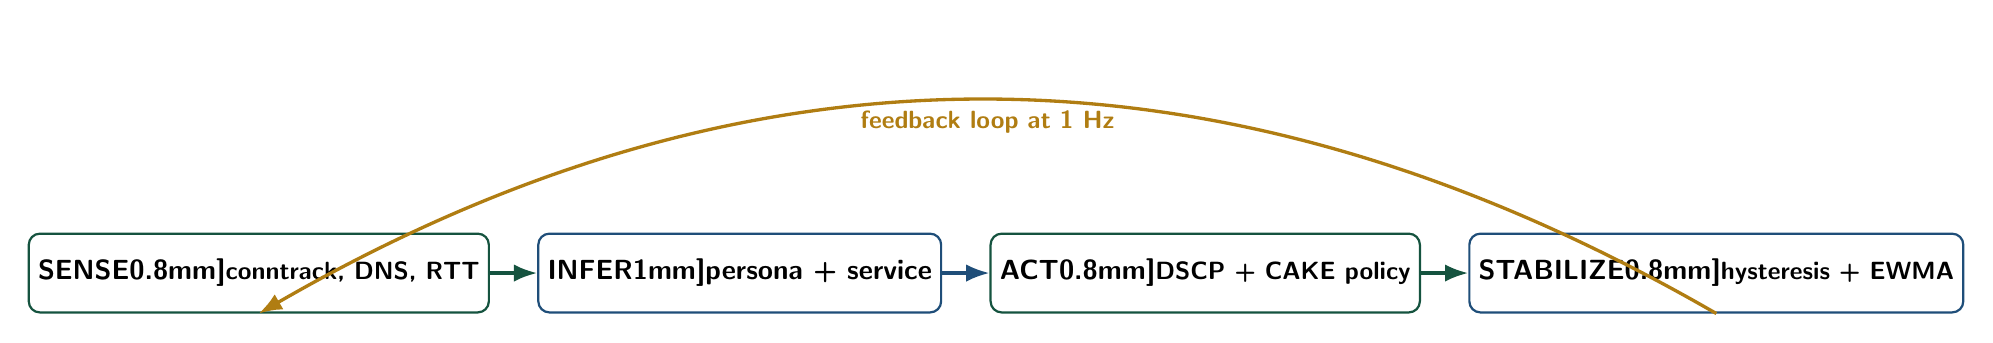
\begin{tikzpicture}[x=1cm,y=1cm,>=Latex, node distance=6mm]
        \node[draw=MycoGreenDark, rounded corners, thick, fill=white, minimum width=2.45cm, minimum height=1.0cm, align=center, font=\bfseries\normalsize] (sense) {SENSE\[0.8mm]\small conntrack, DNS, RTT};
        \node[draw=MycoBlue, rounded corners, thick, fill=white, minimum width=2.45cm, minimum height=1.0cm, align=center, font=\bfseries\normalsize, right=of sense] (infer) {INFER\[1mm]\normalsize persona + service};
        \node[draw=MycoGreenDark, rounded corners, thick, fill=white, minimum width=2.45cm, minimum height=1.0cm, align=center, font=\bfseries\normalsize, right=of infer] (act) {ACT\[0.8mm]\small DSCP + CAKE policy};
        \node[draw=MycoBlue, rounded corners, thick, fill=white, minimum width=2.45cm, minimum height=1.0cm, align=center, font=\bfseries\normalsize, right=of act] (stable) {STABILIZE\[0.8mm]\small hysteresis + EWMA};
        \draw[->, very thick, color=MycoGreenDark] (sense) -- (infer);
        \draw[->, very thick, color=MycoBlue] (infer) -- (act);
        \draw[->, very thick, color=MycoGreenDark] (act) -- (stable);
        \draw[->, very thick, color=MycoGold] (stable.south) to[bend right=30] node[below, font=\bfseries\small] {feedback loop at 1 Hz} (sense.south);
      \end{tikzpicture}%
      

      \vspace{4mm}
      \begin{itemize}[leftmargin=*,itemsep=2pt,topsep=0pt]
        \item \textbf{Classifier signals:} destination port hints, passive DNS observation via \texttt{AF\_PACKET}, and traffic shape.
        \item \textbf{Transport control:} conntrack marks are translated to DSCP values for CAKE diffserv4.
        \item \textbf{RTT guardrail:} passive RTT observation demotes flows when latency exceeds class targets.
      \end{itemize}
    }

    \vspace{2mm}
    \postersection{System footprint}{
      \begin{itemize}[leftmargin=*,itemsep=2pt,topsep=0pt]
        \item Target platform: Xiaomi AX3000T / MediaTek MT7981B
        \item Binary: OpenWrt IPK, C11 daemon, static-pie capable build
        \item Runtime budget: about 9.5\% median daemon CPU in evaluation, 384 KB RSS, zero flash writes
      \end{itemize}
    }
  }
\end{minipage}
\hfill
\begin{minipage}[t]{0.31\textwidth}
  \contentbox{MycoGoldLight}{
    \postersection{Evaluation highlights}{
      \begin{tabular}{@{}p{0.57\linewidth}p{0.34\linewidth}@{}}
        \textbf{Gaming vs. bulk tin delay} & 154$\times$ lower \\
        \textbf{Gaming latency improvement} & 38\% better \\
        \textbf{Observed flow tin accuracy} & 66.97\% \\
        \textbf{Daemon RSS} & 384 KB \\
        \textbf{Flash writes} & 0 \\
      \end{tabular}

      \vspace{3mm}
      \textbf{Key takeaway:} MycoFlow improves QoS by classifying traffic where it is actually observed — on the router — and by converting that decision into CAKE-friendly queue priorities.
    }

    \vspace{3mm}
    \postersection{Deployment status}{
      \begin{itemize}[leftmargin=*,itemsep=2pt,topsep=0pt]
        \item Evaluated in Docker/QEMU and on a live home router.
        \item Supports per-device behavior and per-flow service separation.
        \item Designed to be reproducible: fixed seed, scripted validation, and saved result artifacts.
      \end{itemize}
    }

    \vspace{2mm}
    \postersection{Conclusion}{
      MycoFlow demonstrates that application-aware QoS can run inside a consumer router without cloud dependence or deep packet inspection.
      It is a strong project story for an A1 academic poster because it combines a clear problem, a novel embedded control loop, and measurable network gains.
    }

    \vspace{4mm}
    \begin{center}
      \fcolorbox{MycoGreenDark}{white}{
        \begin{minipage}[c][5.6cm][c]{0.82\linewidth}
          \centering
          {\Large\bfseries Scan / follow-up space}\par
          \vspace{2mm}
          {\large Add a QR code to the repo, demo video, or paper PDF here.}
        \end{minipage}
      }
    \end{center}
  }
\end{minipage}

\vfill

\begin{center}
  {\large\color{MycoGray} MycoFlow Core Poster Draft \quad $\cdot$ \quad A1 landscape \quad $\cdot$ \quad prepared from repository results and documentation}
\end{center}

\end{document}